\newpage
\section{Results and Discussion} \label{sec:results}
The gathered measurements are shown in figures \ref{fig:measurements_pos}, \ref{fig:measurements_neg} and \ref{fig:measurements} (red dots), the calculated value (blue including the shaded uncertainty range) and the best fit (red line). The orange vertical line shows the range of the lock-in frequency.
\begin{figure}[h!]
    \centering
    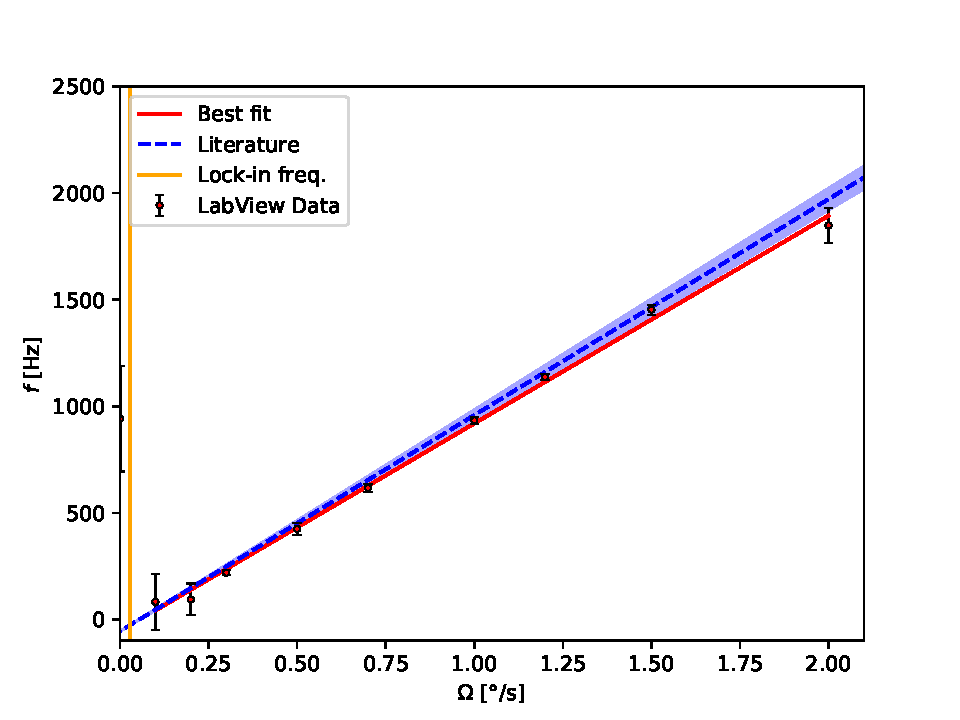
\includegraphics[width=\textwidth]{Gyroscope/Report/plots/slope_pos.pdf}
    \caption{The best fit applied only to the positive velocities. The offset has been added to the theoretically calculated graph.}
    \label{fig:measurements_pos}
\end{figure}
% [1018.30201846  -86.64577303]
% slope = (1018.30 +/- 16.28) krad/deg
% offset = (-86.65 +/- 14.76) krad/s
\begin{figure}[h!]
    \centering
    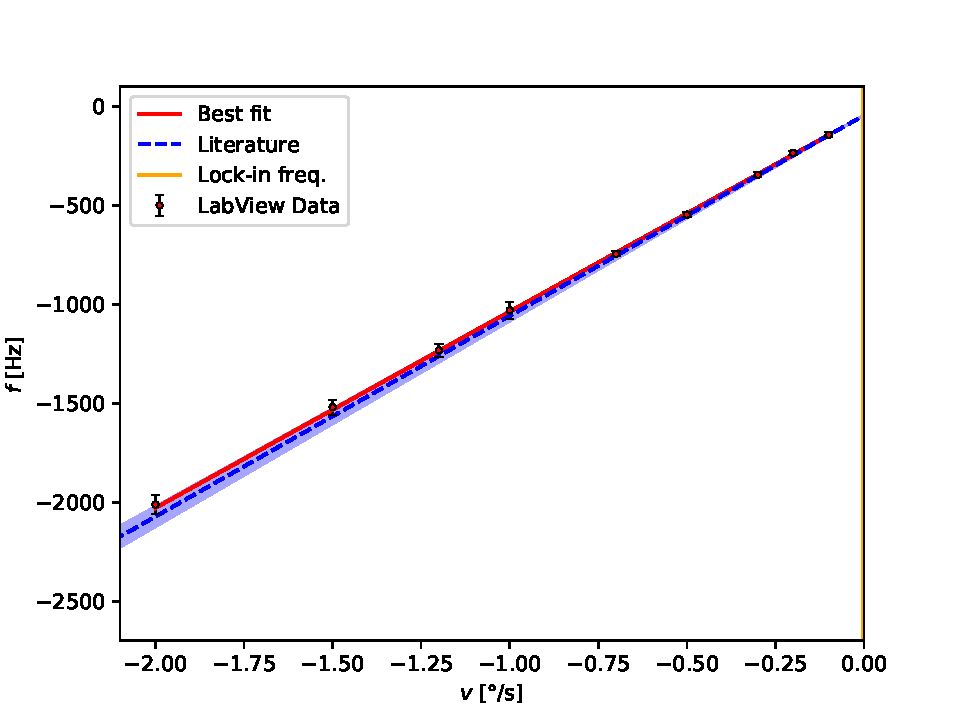
\includegraphics[width=\textwidth]{Gyroscope/Report/plots/slope_neg.pdf}
    \caption{The best fit applied only to the negative velocities. The offset has been added to the theoretically calculated graph.}
    \label{fig:measurements_neg}
\end{figure}
% dt = 1 ms on oscilloscope:
% [991.66875925 -45.93399194]
% slope = (991.67 +/- 14.88) krad/deg
% offset = (-45.93 +/- 8.37) krad/s
\begin{figure}[h!]
    \centering
    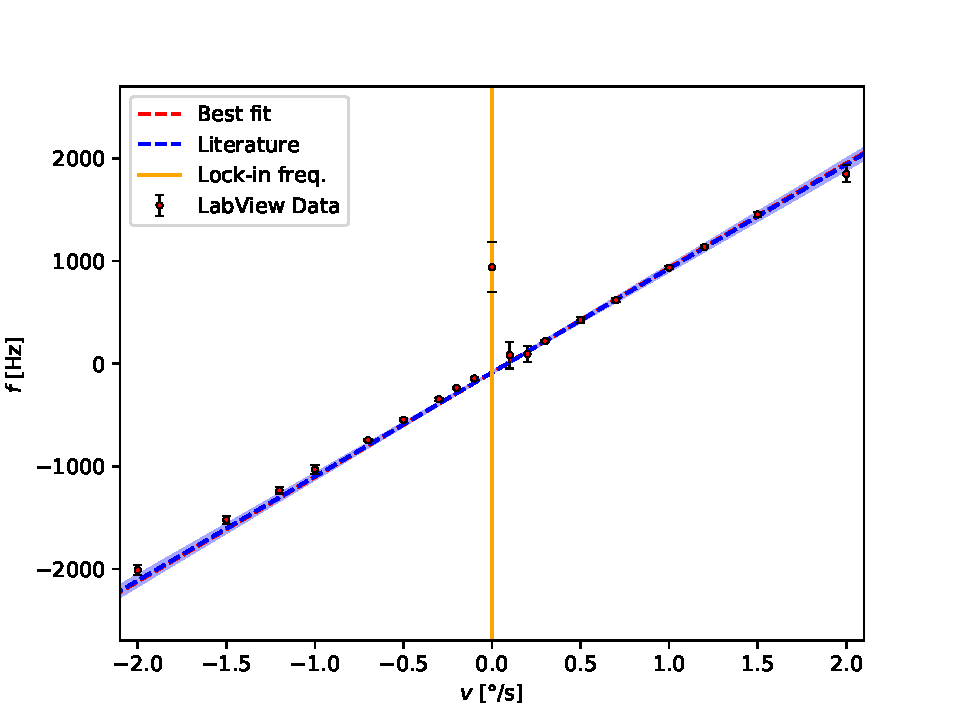
\includegraphics[width=\textwidth]{Gyroscope/Report/plots/slope.pdf}
    \caption{The best fit applied to all data-points. The offset has been added to the theoretically calculated graph.}
    \label{fig:measurements}
\end{figure}
% [983.9798354  -52.58991876]
% slope = (983.98 +/- 5.86) krad/deg
% offset = (-52.59 +/- 4.14) krad/s
The theoretically calculated value using equation \ref{eq:slope} is:
$$\Delta \nu = (1013.43 \pm 25.34)\, \Omega $$
The values from the fits to the measurements are given in table \ref{tab:measurements}:
\begin{table}[h!]
\centering\begin{tabular}{l|c|c}
\hline direction & $\Delta \nu$ & offset \\ \hline
     ccw & $1018.30 \pm 16.28$ & $-86.65 \pm 14.76$\\
     cw & $991.67 \pm 14.88$ & $-45.93 \pm 8.37$ \\
     both & $983.98 \pm 5.86$ & $-52.59 \pm 4.14$
\end{tabular}
\caption{Calculated parameters from the fit.}
\label{tab:measurements}
\end{table}
